%%%%%%%%%%%%%%%%%%%%%%%%%%%%%%%%%%%%%%
% Contribution to IKP annual report 2021
%%%%%%%%%%%%%%%%%%%%%%%%%%%%%%%%%%%%%%
\documentclass[fleqn,twocolumn,a4paper]{ikpar}
\usepackage{hyperref}
\usepackage{paralist}
\usepackage{times,mathptm}
\usepackage{graphicx}
\usepackage{float}
\usepackage{stfloats}
\usepackage{caption}
\usepackage{subfig}
\usepackage{gensymb}
\pagestyle{empty}

% standadized SI units
\usepackage[per-mode=symbol, range-units=single, binary-units=true]{siunitx}
\DeclareSIUnit\clight{\text{\ensuremath{c}}} % redefine light speed symbol
\DeclareSIUnit\momentum{\GeV\per\clight} % momentum in GeV/c
\DeclareSIUnit\tmom{(\momentum)^2} % 4-momentum squared
\DeclareSIUnit\atom{\text{atoms}} 
\DeclareSIUnit\event{\text{events}} 

% \addtolength{\topmargin}{-0.2cm}
% \addtolength{\textheight}{0.2cm}
\begin{document}
\parindent=0pt
\frenchspacing

\title{{\bf
    Determination of the Cluster Target Density Profile in KOALA
}}
\author{Yong Zhou
}

\maketitle

%%%% Background, problem description, topic and results of this report
KOALA aims to measure the differential cross section of (anti)proton-proton elastic
scattering over a wide $|t|$ range from \SIrange{0.0008}{0.1}{\tmom}.
In the initial setup, in which only the recoil detector was in operation, the high yield of low-energy
background deteriorates the elastic peak identification at small recoil angles and limits the lower measurement range of KOALA.
The forward detector, which consists of fast scintillators, has been
commissioned in 2019 to help suppress the low energy background based on the TOF-E
relation of the recoil protons.
The design of the forward detector has been verified in the following test runs and energy spectra from pure elastic scattering events can now be obtained after the TOF-E selection.
Due to the lower limit of the acceptance of the forward detector, the spectra
of strips at very small recoil angles start to lose events from the
target volume below a threshold angle.
However, it is found that this phenomenon already appears at a larger recoil angle than the design goal.
% This may be caused by the large thickness of the cluster target along the beam axis.
More accurate information about the target profile is needed to clarify this phenomenon.
In this report, a new method of determining the density profile of the cluster
target is described, and the result from the 2019 test is presented.
Implications of the measured target profile on the lower limit of KOALA measurement range is also discussed.

\begin{figure*}[b]
  \centering
	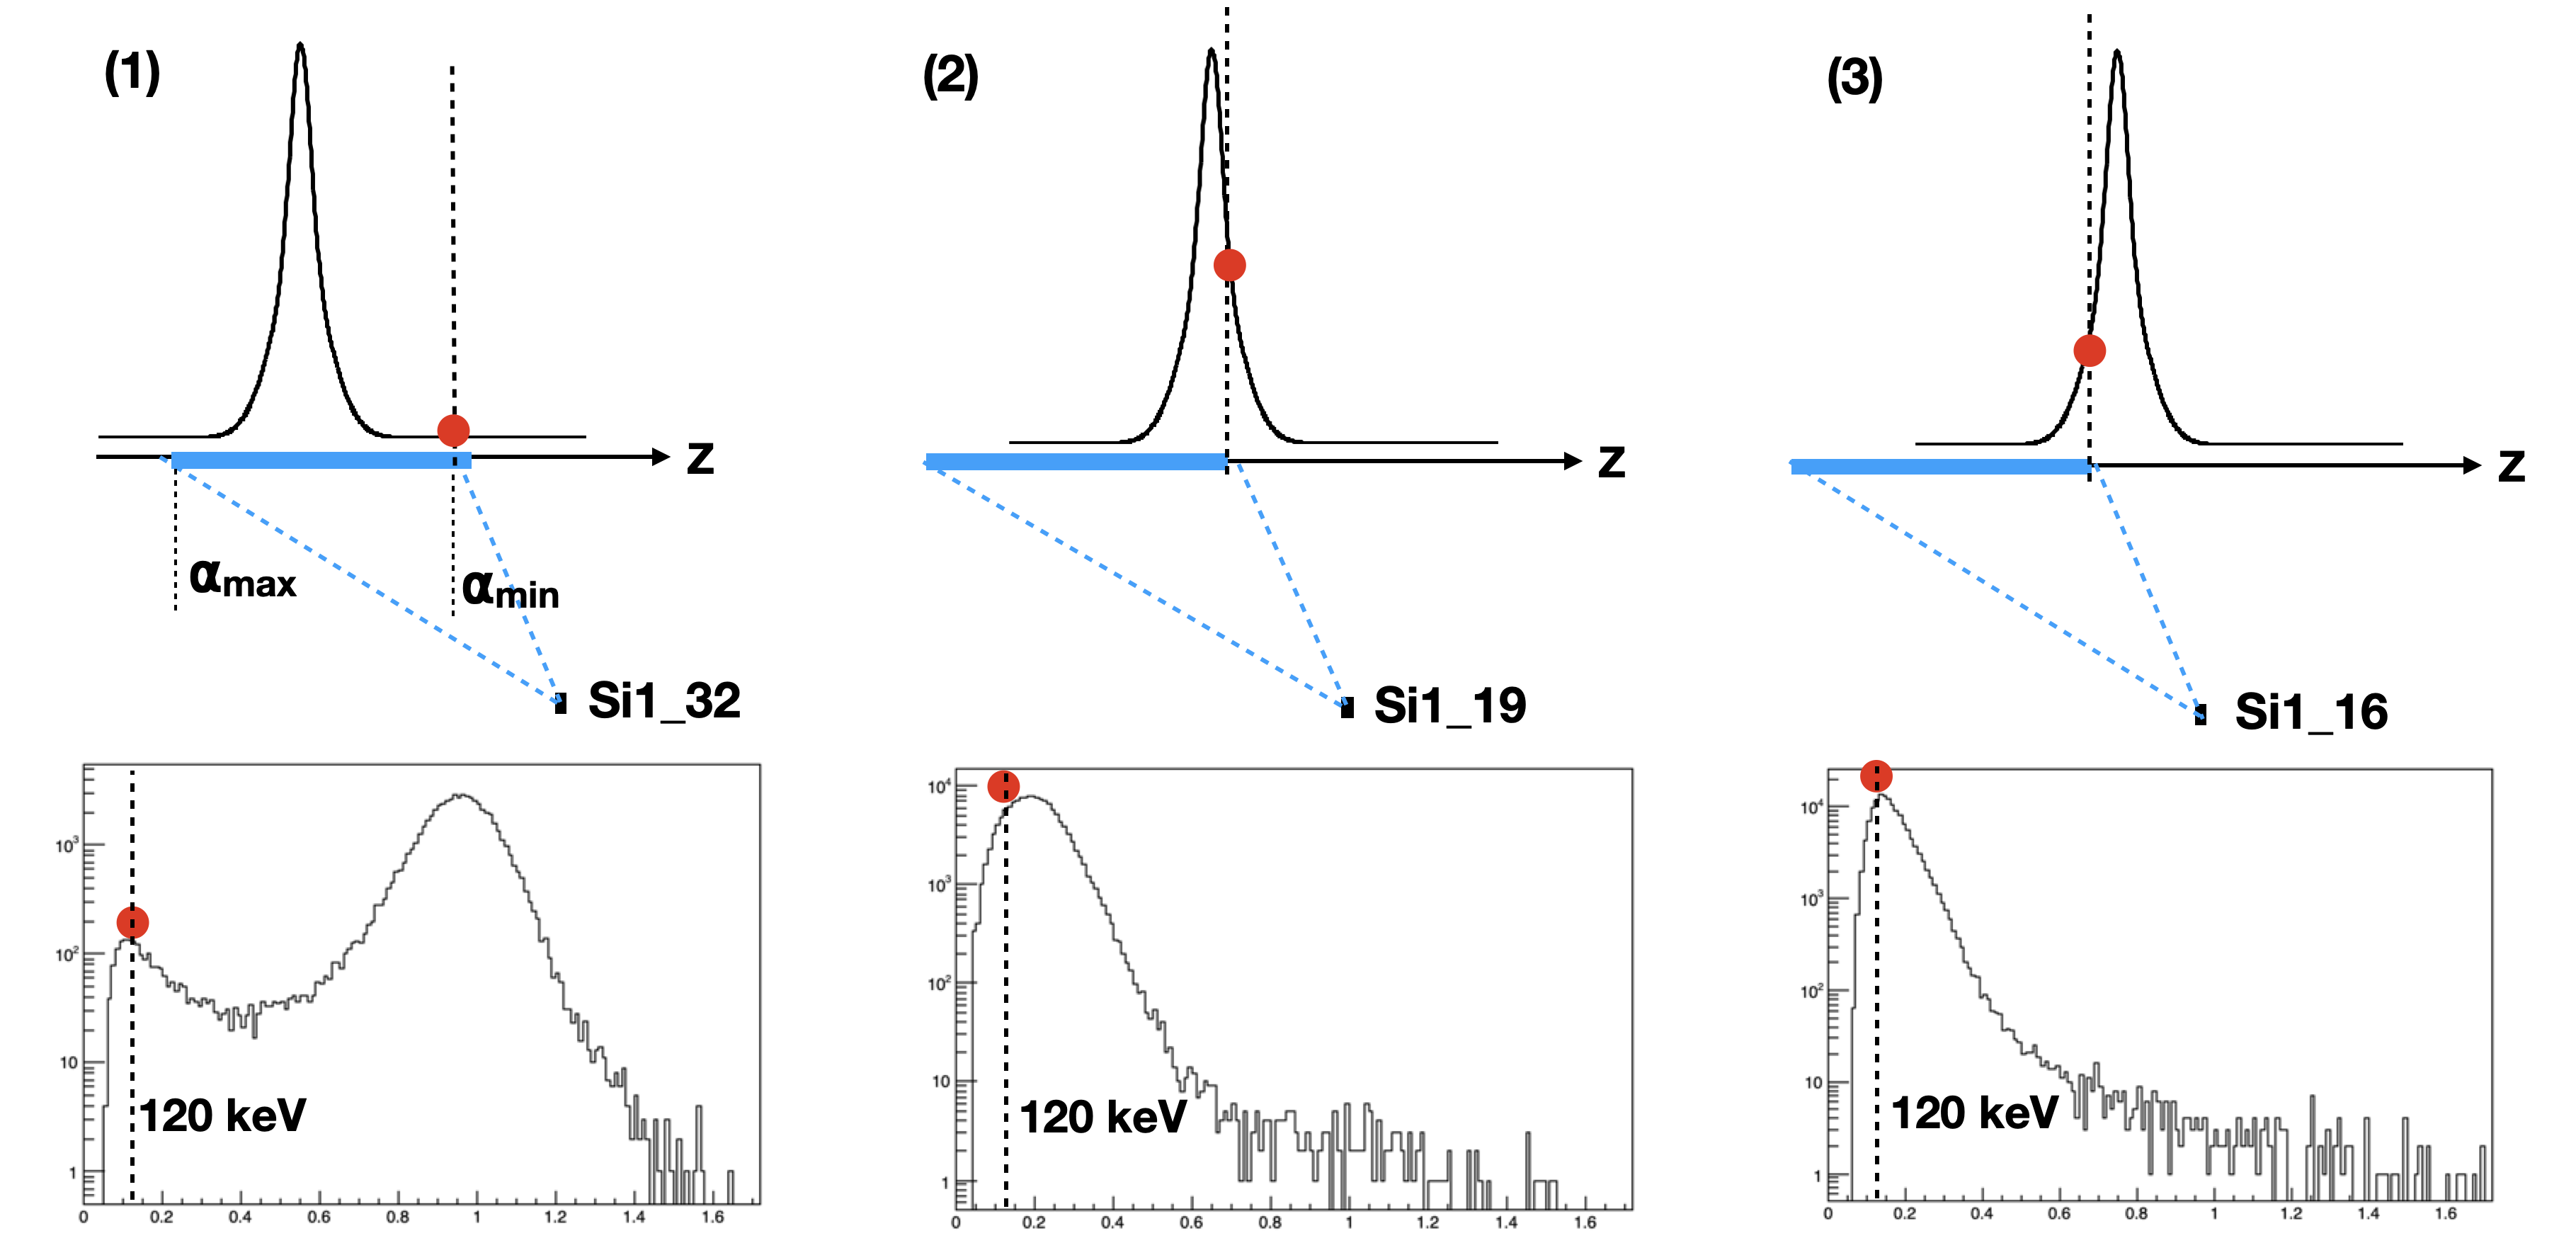
\includegraphics[width=0.8\textwidth]{./target_density_determination.png}
  \caption{Elastic energy spectra measured by three strips at different recoil
    angles: (1) the full target volume is within the Forward Detector acceptance; (2) part of the target volume is not within the
  acceptance, but the center of the target volumn is still whitin the
  acceptance; (3) the target center is outside of the acceptance, only the tail
  of the target profile is recorded. The first row shows the target profile
  shape and the second row shows the energy spectrum.
  % The blue bar indicates the
  % region along the beam axis that is in the joint acceptance of the given strip
  % in the recoil detector and the forward detector.
  The red dot indicates the reference energy bin and its corresponding position in the target profile.}
  \label{fig:target_density_determination}
\end{figure*}

\par
\medskip

%%%%% Description of the method
Three scenerios are depicted in Fig. \ref{fig:target_density_determination} to
show the variation of the TOF-E selected energy spectra from strips at descreasing recoil angles.
The acceptance of the forward detector are represented by the recoil angle as
$[\alpha_{min}, \alpha_{max}]$, which in turn can be converted to a region
before the strip as indicated by blue bars in Fig. \ref{fig:target_density_determination}.
Elastic scattering events from this region will hit both the recoil detector and the
forward detector and generate coincidences.
% The length of the region are roughly the same for different strips, since the interaction point is far away (\SI{4.6}{\m}) from the interaction point.
% The change of $\alpha_{min}$ and $\alpha_{max}$ is very small for different
% positions along the beam axis, since the interaction point is far way (\SI{4.6}{\m}) from the interaction point.
Starting from a strip which covers the full target volume (Fig.
\ref{fig:target_density_determination} (1)), part of the target volume gradually
fall out of the acceptance region as approaching to the interaction point (Fig.
\ref{fig:target_density_determination} (2)), then the peak, and finally only the
tail of the target is covered (Fig. \ref{fig:target_density_determination} (3)).
Strips that are further upstream no longer have a coincidence with the forward detector for events in the beam-target overlap volume.
Instead only events occuring in the rest-gas within the beam pipe generate coincidences.

\par
\medskip

The number of TOF-E selected elastic scattering events $N_{elastic}$ recorded on a single recoil strip has the
following relation with other experiment parameters,
\begin{equation}
  N_{elastic} = \epsilon_{DAQ}\cdot l_{beam}\cdot\rho_{target}\cdot\sigma_{elastic}\cdot\epsilon_{acceptance}.
\end{equation}
where $\epsilon_{DAQ}$ is the DAQ efficiency, $l_{beam}$ is the beam intensity, $\rho_{target}$ is the target density,
$\sigma_{elastic}$ is the cross section of elastic scattering and
$\epsilon_{acceptance}$ is the acceptance of the forward detector.
$l_{beam}$ and $\epsilon_{DAQ}$ are constant in the same run.
To determine $\rho_{target}$, the last two items $\sigma_{elastic}$ and
$\epsilon_{acceptance}$ need to be fixed.
$\sigma_{elasitc}$ is determined by the energy of the recoil proton, thus can be
fixed by choosing the same energy value as reference.
$\epsilon_{acceptance}$ varies with the recoil angle as well as the beam size.
Simulation shows that strips at the lower range of the forward coverage are
guaranteed to be fully covered as long as the width of the beam profile is
smaller than \SI{10}{\mm}, see Fig. \ref{fig:fwd_acceptance}.
The estimated width of the beam profile of COSY is about \SI{7}{\mm}.
Since each strip corresponds to a specific recoil angle which in turn
can be converted to an energy value, this indicates that the elastic events with
energy near the edge the TOF-E selected energy spectrum are guaranteed to be
fully covered and have $\epsilon_{acceptance} \approx 1$.
\begin{figure}[t!]
  \centering
	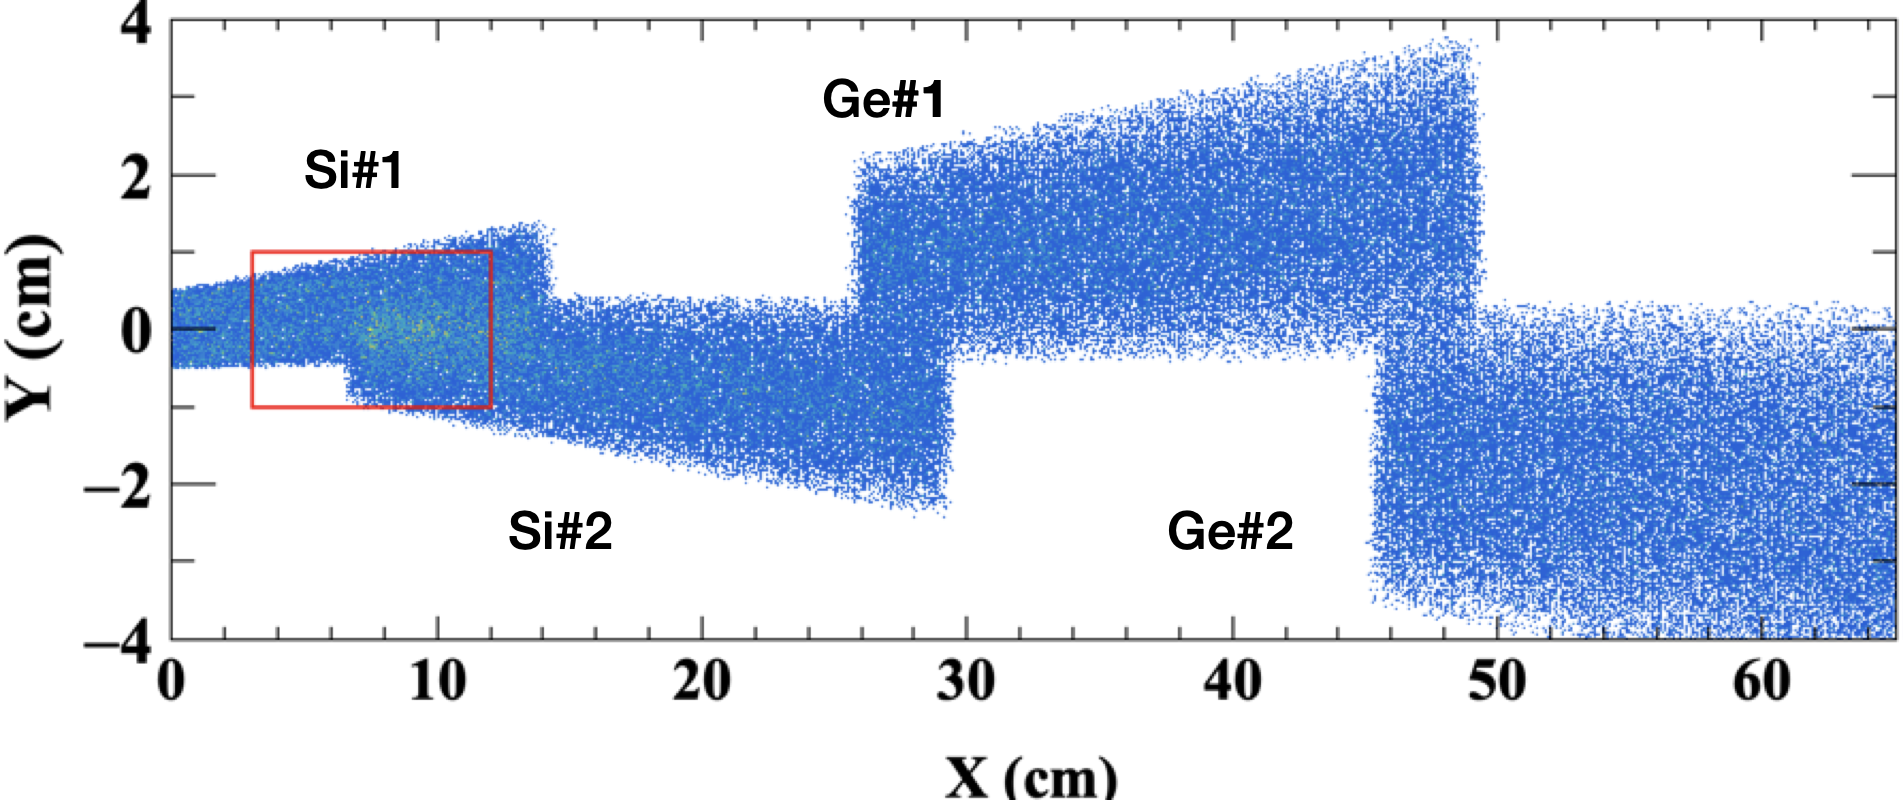
\includegraphics[width=0.5\textwidth]{./fwd_acceptance.png}
  \caption{
    Hit positions of the forward scattered particle on a plane at
    $z=\SI{4.6}{\m}$ that are coincident with a recoil particle hitting one of
    the four recoil sensors. The beam is assumed to have a width of \SI{10}{\mm}.
     The red square indicates the size of the forward scintillators.}
  \label{fig:fwd_acceptance}
\end{figure}
Thus, the number of events in these energy bins provides a direct measurement of the target density.

The observed lower limit of the forward acceptance is about \SI{100}{\keV} for
the data collected with $P_{beam} = \SI{2.2}{\GeV}$, as shown in Fig. \ref{fig:spectrums}.
The value is consistent with the calculated range of the forward detector's
acceptance with ideal beam condition, which is from \SIrange{0.096}{1.56}{\MeV}.
Thus, \SI{120}{keV} with bin width of \SI{10}{\keV} is selected as the
measurement reference.
The target density distribution along the beam axis is obtained by recording the
number of events at a given energy bin in all strips.
The reference energy is then converted back to a position before the strip center
(at \SI{2.2}{\momentum} beam momentum, \SI{120}{\keV} corresponds to $z=\SI{10}{\mm}$).
\par
\medskip

Two independent methods are used to deduce the position distribution of the density profile.
The first method is based on the strip position in the ideal geometry model.
This method gives the distribution in the laboratory reference frame.
The second method is based on the energy difference of the reference energy and
the peak energy.
\begin{figure}[b!]
  \centering
	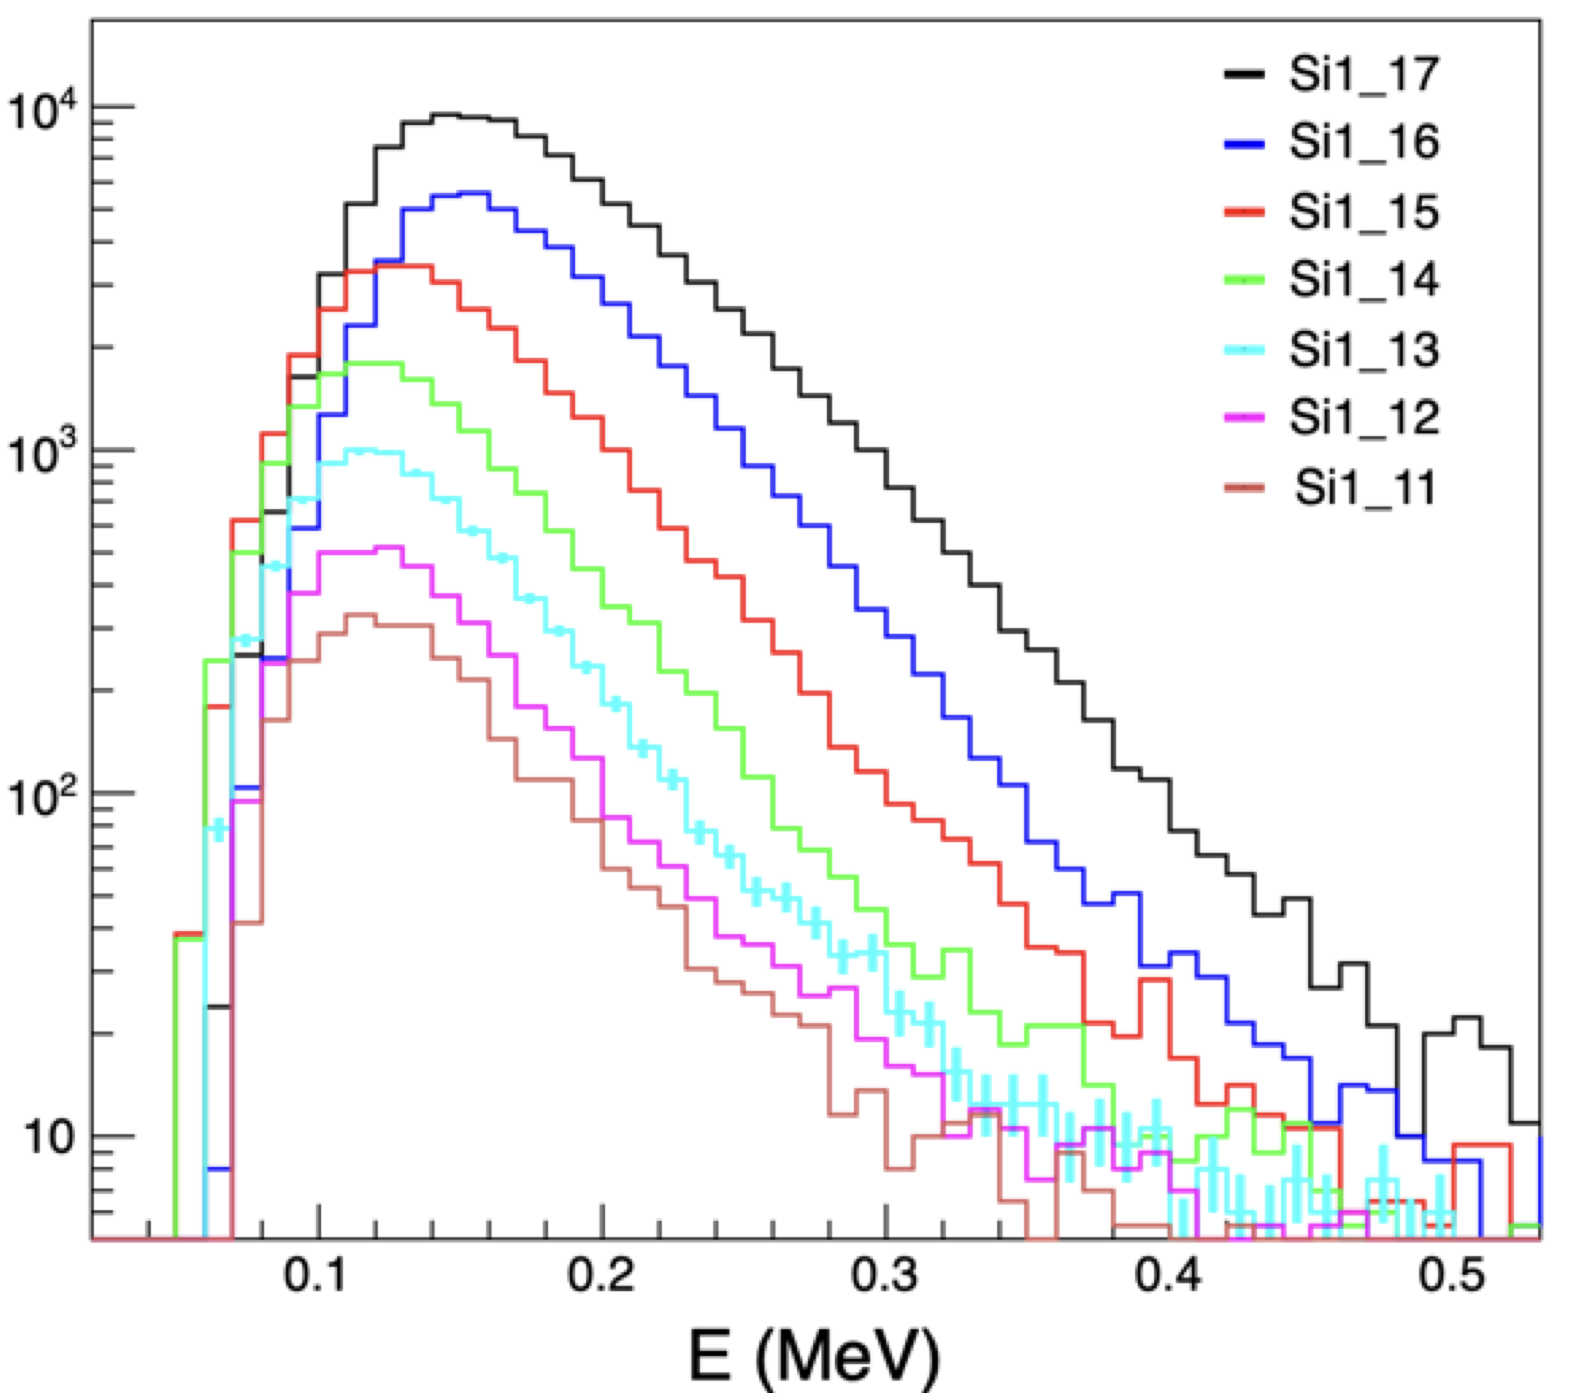
\includegraphics[width=0.4\textwidth]{./spectrums.png}
  \caption{TOF-E selected energy spectra from several strips that only cover the tail of the target volume. The lower limit can be clearly identified.}
  \label{fig:spectrums}
\end{figure}
The elastic energy peak corresponds to the target density center.
Thus, the energy difference can be converted to a position relative to the target center. 
This method gives the distribution in the reference frame where the
target center is at the origin.
However, it is limited by the requirement of the coverage of the target center
and only gives the first half of the density distribution.
\begin{figure}[t!]
  \centering
	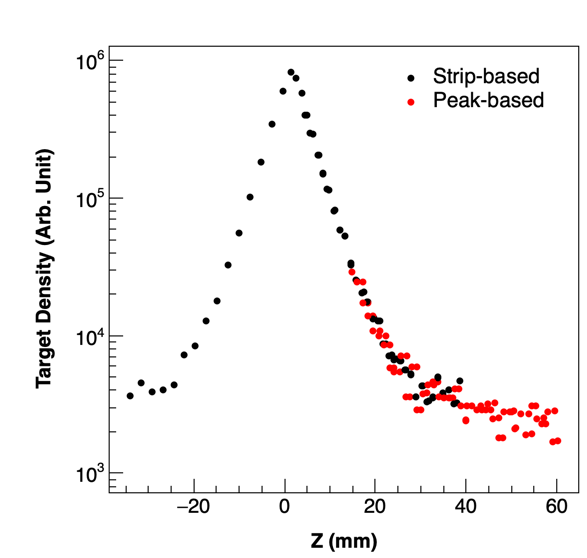
\includegraphics[width=0.35\textwidth]{./target_density_result.png}
  \caption{Target density profile measured at \SI{2.2}{\momentum}. The black
    data points are from the first method, the red data points are from the
    second method. They are aligned with each other after a \SI{1.8}{\mm} shift of
    the recoil sensors along the beam axis.}
  \label{fig:target_density_result}
\end{figure}
The comparison between the results from the two methods can be used to align the the recoil detector to the target center.

\par
\medskip

%%%%% Discussion of the results
Fig. \ref{fig:target_density_result} shows the target density profile measured at
\SI{2.2}{\momentum}.
The distribution is almost symmetric with respect to the target center.
The main target volume lies above a wide spread of residual gas.
The main volume can be described by a double-gaussian model, with
\SI{43}{\percent} and \SI{57}{\percent} contribution from the narrow and wide
component, respectively.
The narrow component has $\sigma = \SI{2}{\mm}$ and the wide one has $\sigma = \SI{5.6}{\mm}$.
The overall FWHM of the target profile is about \SI{6.9}{mm}.
The residual gas has a relatively uniform distribution over a wide region, even
beyond the recoil sensor's coverage.
The density of the residual gas is about a factor 260 lower than the peak density of the target.

\par
\medskip

The measured target density distribution is much wider than the design value of \SI{2}{\mm} FWHM.
However, the deduced density is an integrated value over the X-Y plane, thus
may be afftected by the finite angular dispersion of the beam.
Correspondingly, the TOF-E selection method reaches its lower limit at larger recoil angle than the design goal.
At $P_{beam}=\SI{2.2}{\momentum}$, the target volume is not fully covered by
the forward detector starting from the strip Si1\_26.
This corresponds to the recoil energy of \SI{500}{\keV} and $|t| \approx \SI{0.001}{\tmom}$.
The background subtraction method using the background model from strips which
are fully covered by the forward detector can extend the lower limit to $|t| \approx \SI{0.0006}{\tmom}$.
However, this method has larger systematic error than the TOF-E selection method.
Finally, to reach even lower $|t|$, new methods need to be developed to unfold the
actual event rate from the partially-recorded energy spectrum.

\par
\medskip

%----------------------------------------------------------------
\begin{thebibliography}{99}
\bibitem{r1} Y. Zhou, Extraction of elastic scattering events in KOALA, IKP Annual Report 2021.
\end{thebibliography}
\end{document}

